\chapter{Cutflow Studies}\label{app:cutflows}

This appendix shows further studies on signal selection efficiency. 

\noindent \textbf{Resonant Signal Yield}\\
\indent The relative and absolute selection efficiency after each cut for the resonant samples is shown in Figure~\ref{fig:resonant-cutflow-1tag} for the 1 \btag category, and in Figure~\ref{fig:resonant-cutflow-0tag} for the 0 \btag category, for both the low and high mass selections, as indicated.


%%% Resonant cutflows

\begin{figure}[!b]
    \centering
    \subfloat[Low Mass Selection]{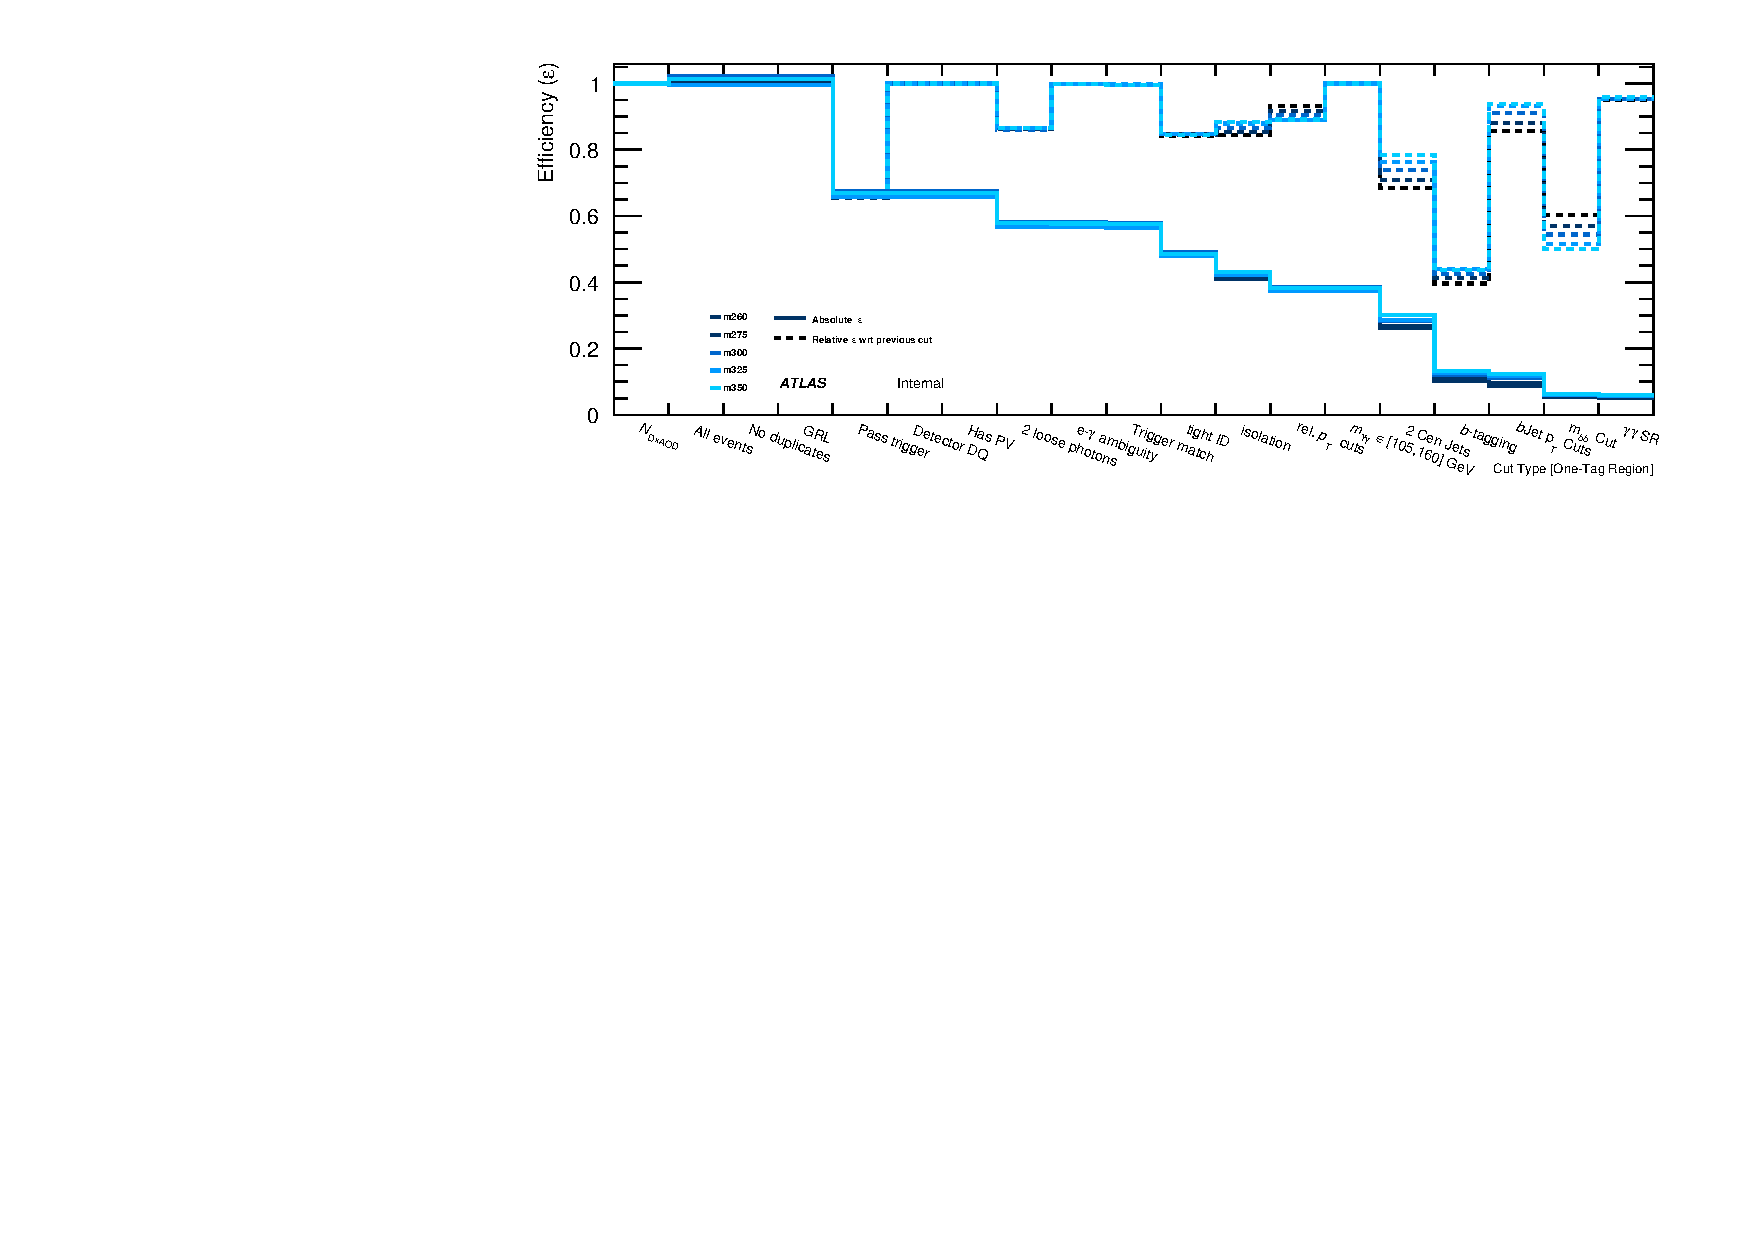
\includegraphics[width=\textwidth]{appendices/cutflows/OneTag_EfficiencyOverlay_LowMass.pdf}}\\
    \subfloat[High Mass Selection]{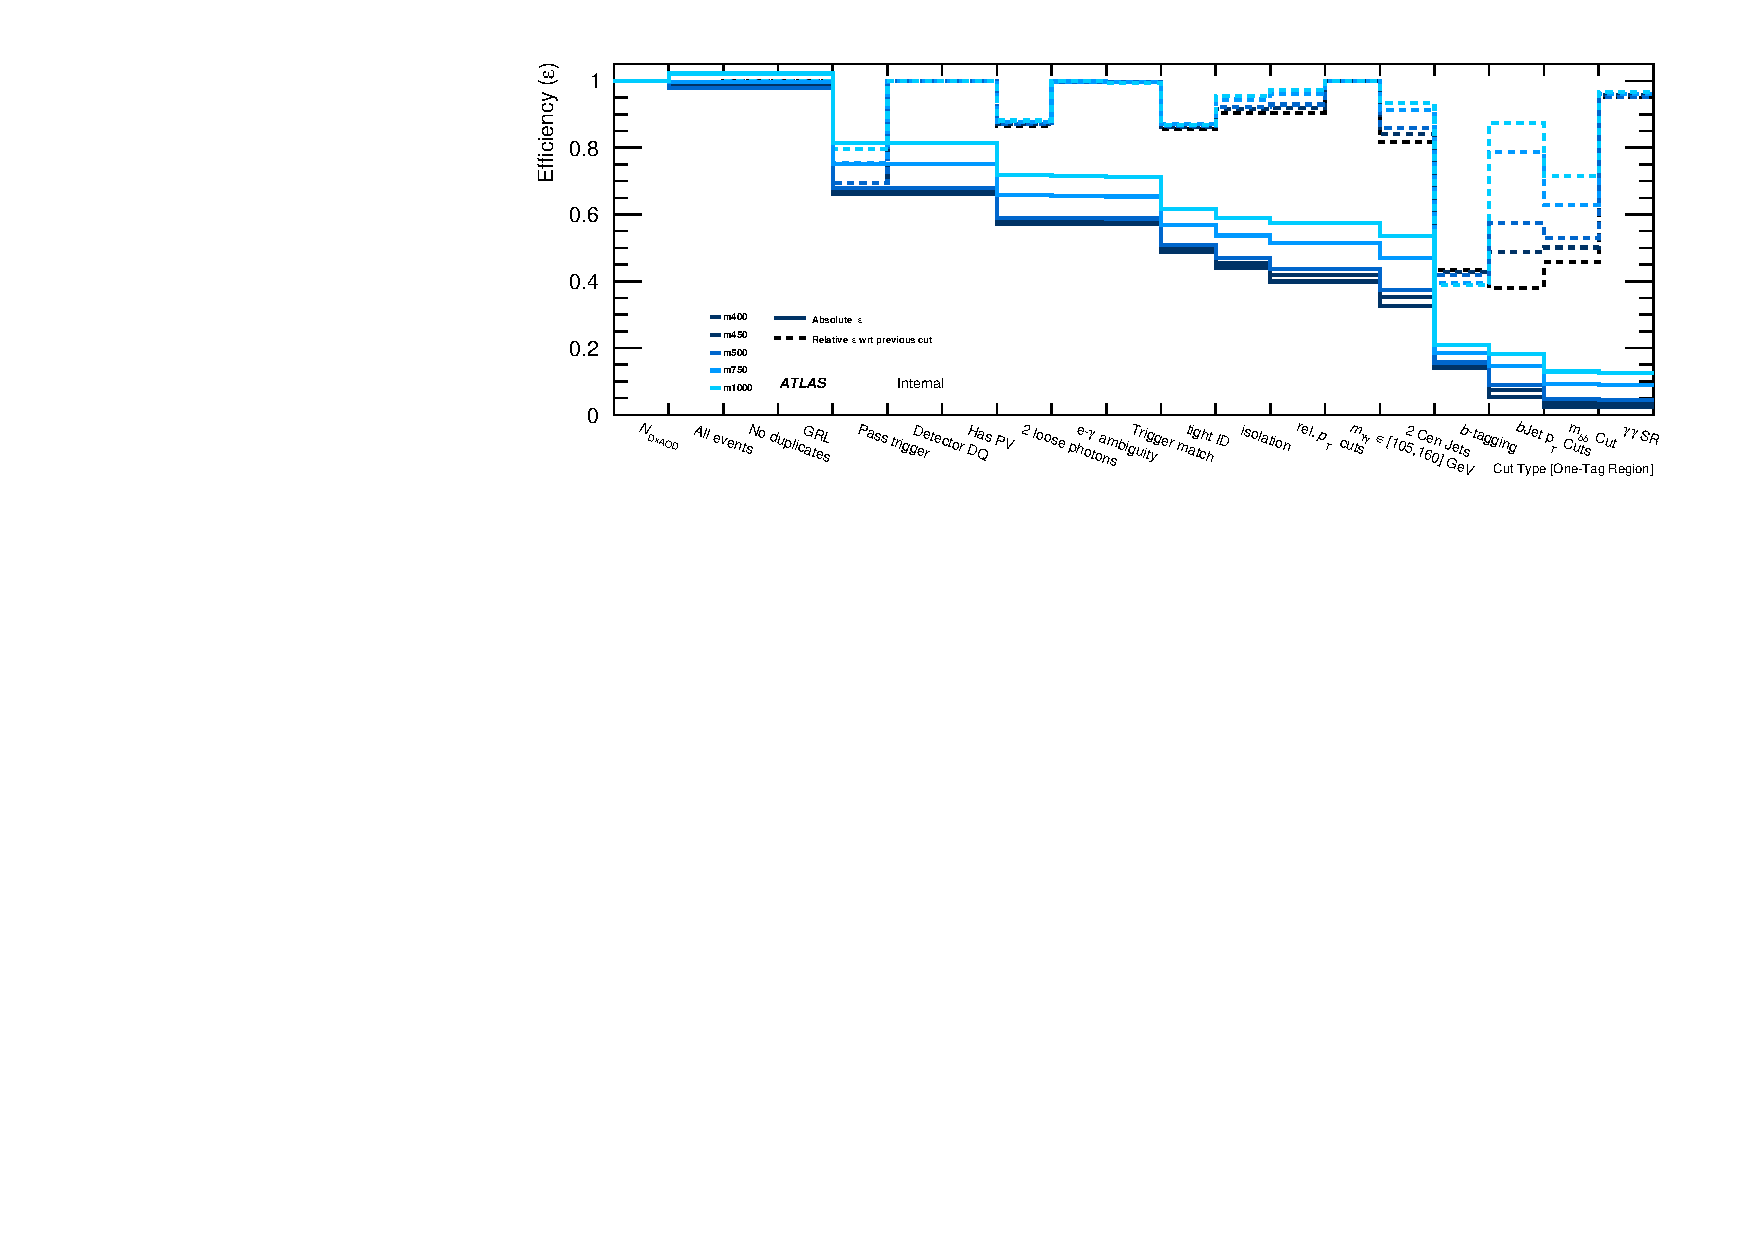
\includegraphics[width=\textwidth]{appendices/cutflows/OneTag_EfficiencyOverlay_HighMass.pdf}}
    \caption[Absolute and relative efficiencies for the 1 \btag category, high mass selection]{Absolute (solid line) and relative (dotted line) efficiencies for the 1 \btag resonant signal samples to pass each cut in the low (a) and high (b) mass selection}
    \label{fig:resonant-cutflow-1tag}
  \end{figure}


\clearpage

\begin{figure}[!b]
    \centering
    \subfloat[Low Mass Selection]{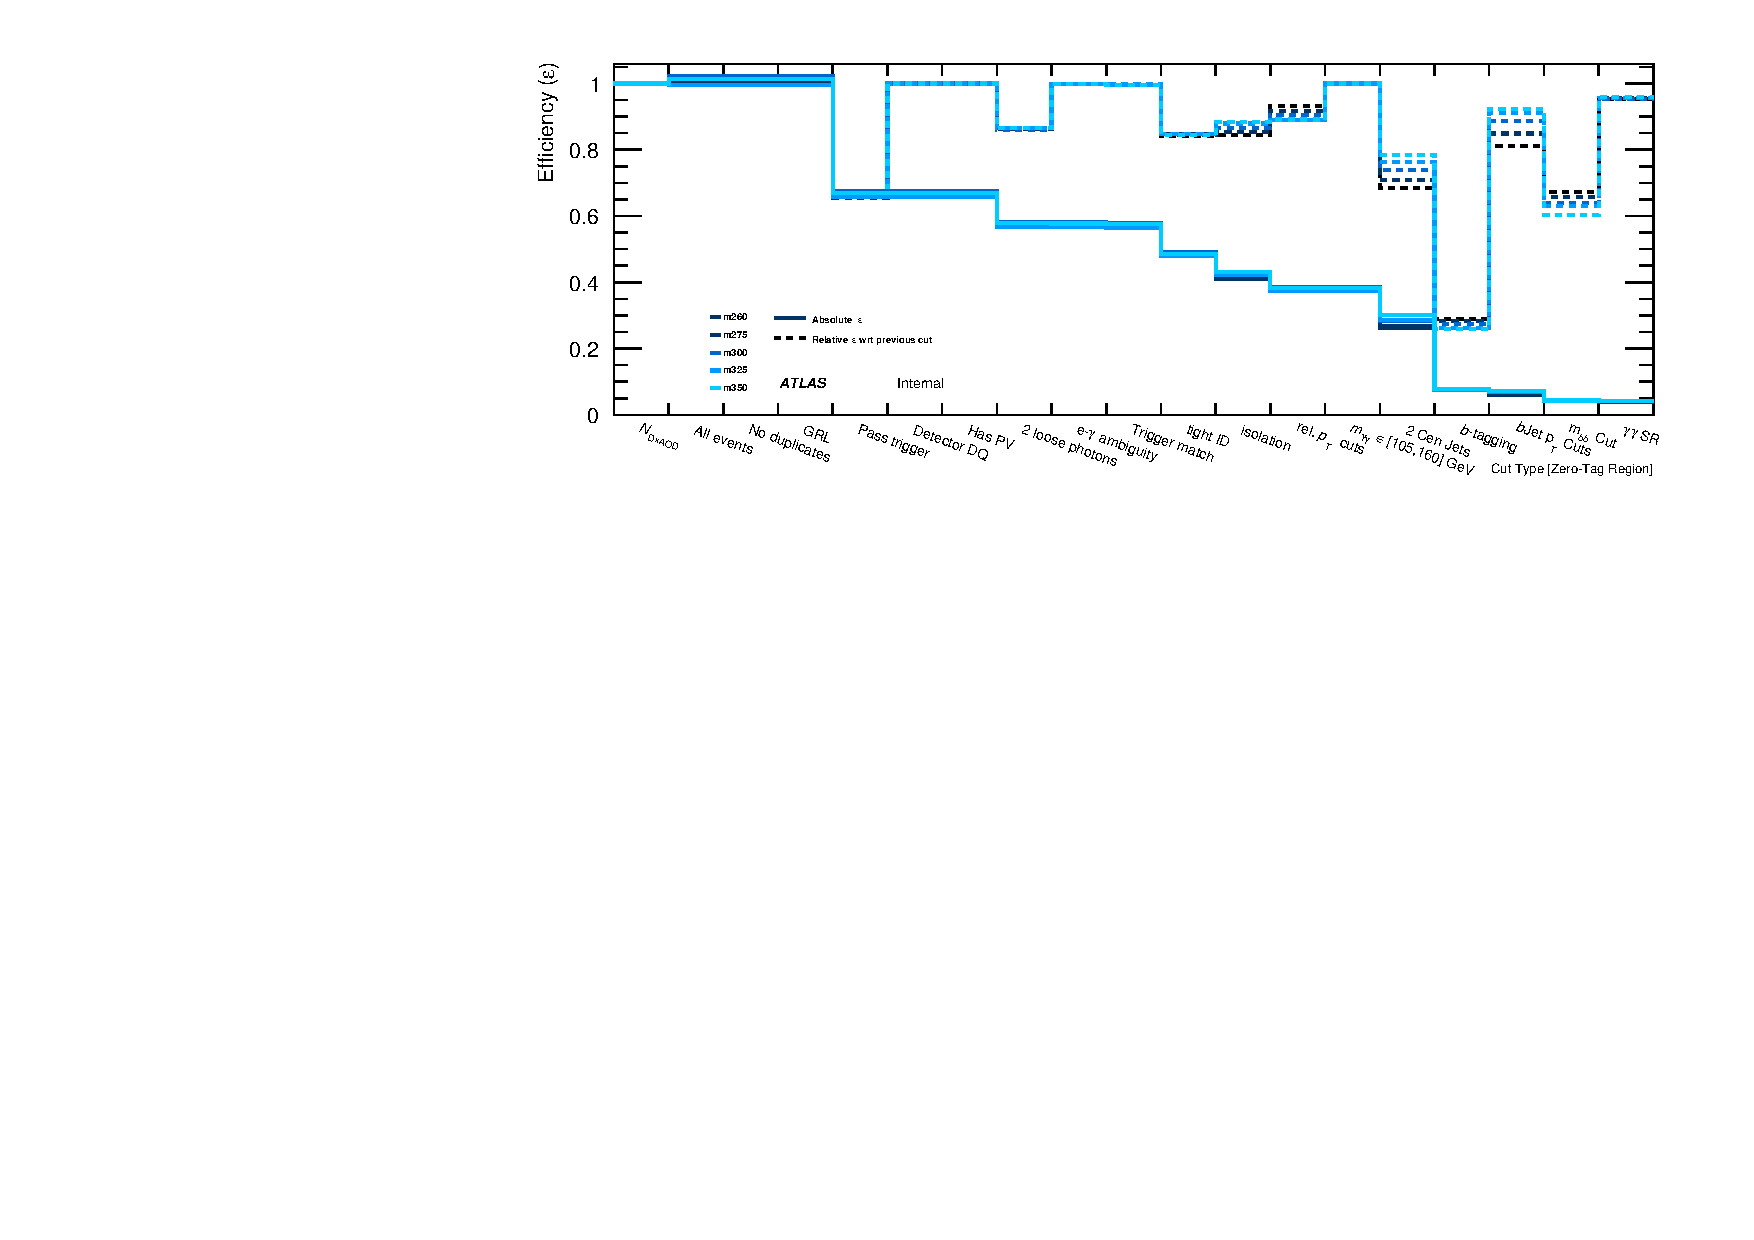
\includegraphics[width=\textwidth]{appendices/cutflows/ZeroTag_EfficiencyOverlay_LowMass.pdf}}\\
    \subfloat[High Mass Selection]{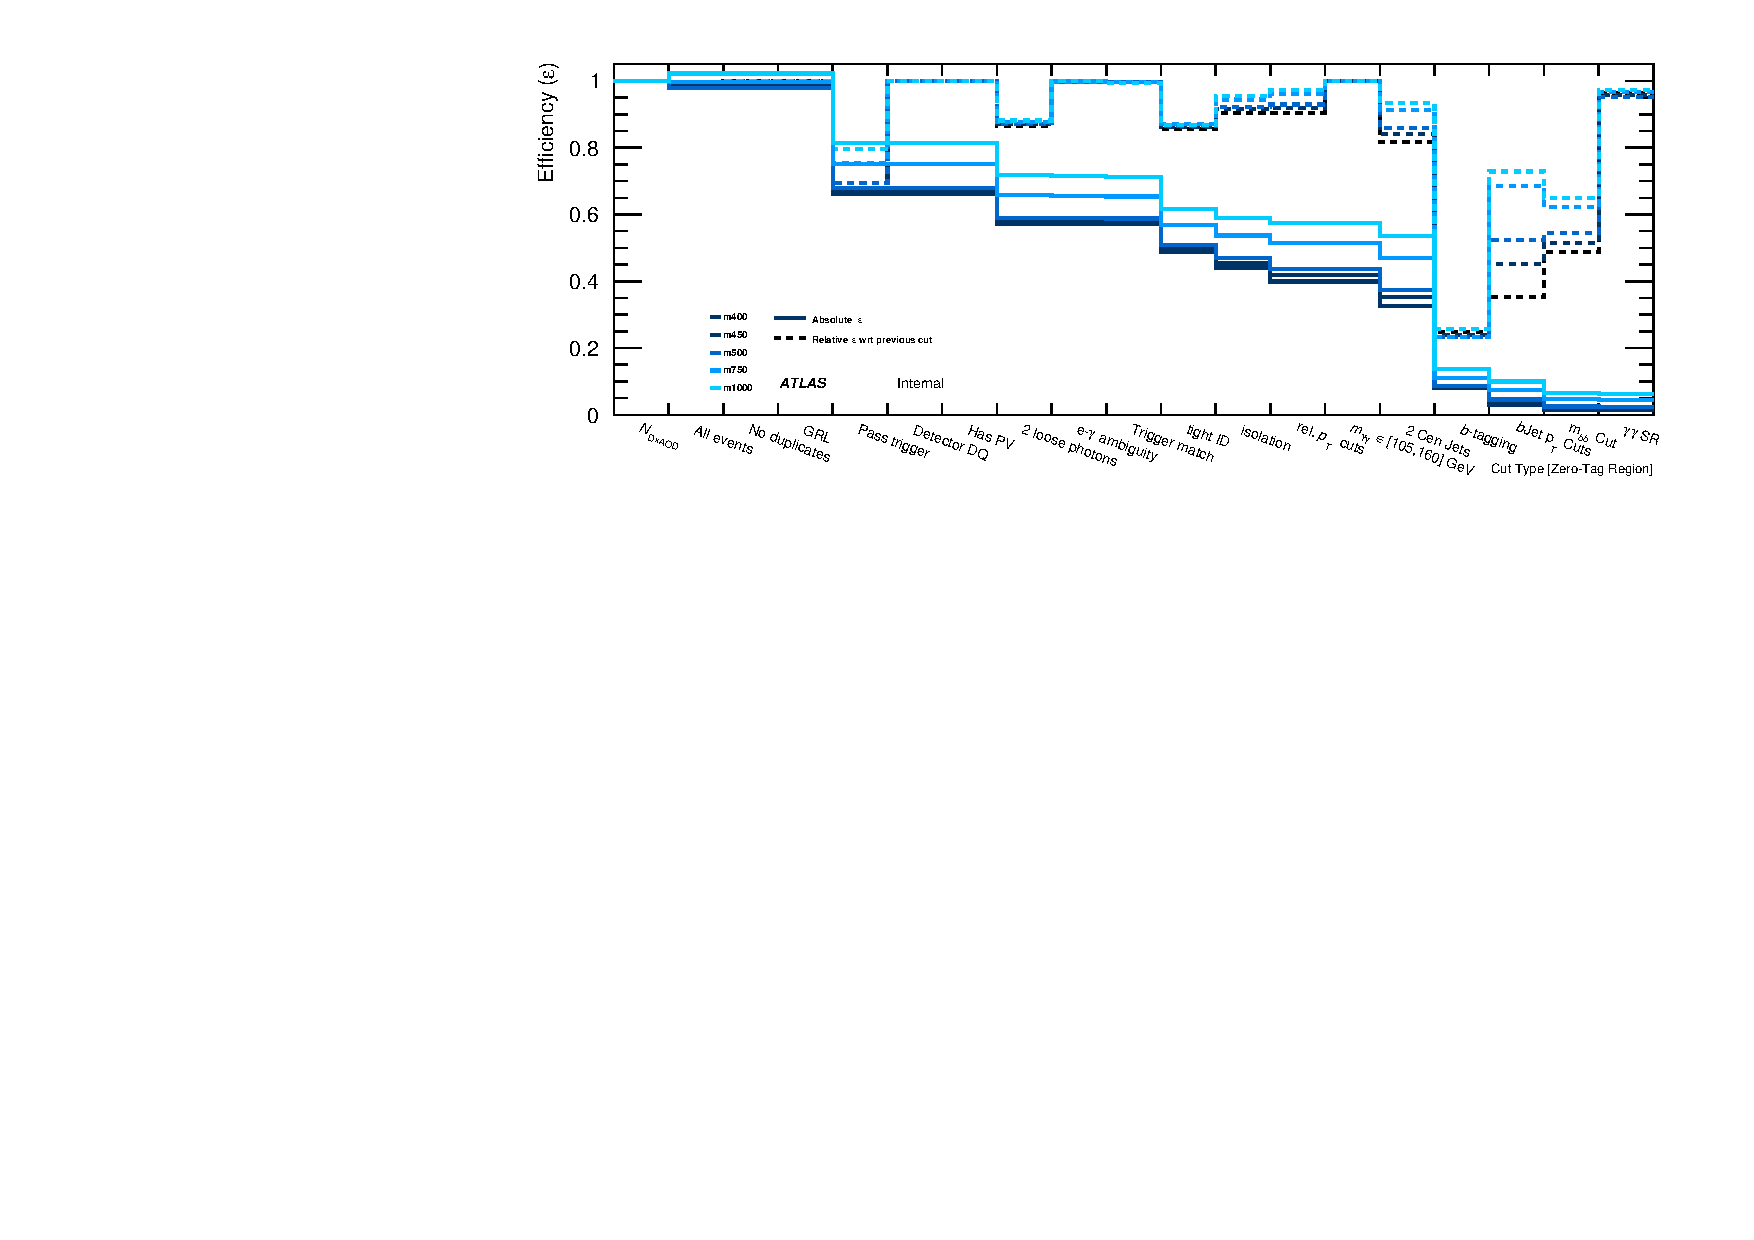
\includegraphics[width=\textwidth]{appendices/cutflows/ZeroTag_EfficiencyOverlay_HighMass.pdf}}
    \caption[Absolute and relative efficiencies for the 0 \btag category, high mass selection]{Absolute (solid line) and relative (dotted line) efficiencies for the 0 \btag resonant signal samples to pass each cut in the low (a) and high (b) mass selection}
    \label{fig:resonant-cutflow-0tag}
  \end{figure}


\clearpage

%%% nonresonant cutflows


\noindent \textbf{Non-Resonant Signal Yield}\\
\indent The yield and efficiency for each successive analysis cut are shown in Tables~\ref{tab:cutflow-nonres-1tag-low},~\ref{tab:cutflow-nonres-1tag-high},~\ref{tab:cutflow-nonres-0tag-low}, and~\ref{tab:cutflow-nonres-0tag-high} for the 1 \btag low mass, 1 \btag high mass, 0 \btag low mass, and 0 \btag high mass selections respectively.

\begin{table}\footnotesize
\begin{center} 
\caption{Cutflow for non-resonant \hhyybb, 1 tag category (low mass selection)}
\label{tab:cutflow-nonres-1tag-low}
\begin{tabular}{|c|c|c|c|} 
 \hline 
Cuts& \multicolumn{3}{c|}{1 b-tag} \\ \hline 
 &Yield&Error&Efficiency\\ \hline 
$N_{xAOD}$ & 3.147&0.027 &$-$ \\ 
 \hline 
$\it{N}_{DxAOD}$ & 3.147&0.019 &$-$ \\ 
 \hline 
$All\ events$ & 3.181&0.024 &100.0 \\ 
 \hline 
$No\ duplicates$ & 3.181&0.024 &100.0 \\ 
 \hline 
$GRL$ & 3.181&0.024 &100.0 \\ 
 \hline 
$Pass\ trigger$ & 2.184&0.021 &68.7 \\ 
 \hline 
$Detector\ DQ$ & 2.184&0.021 &68.7 \\ 
 \hline 
$Has\ PV$ & 2.184&0.021 &68.7 \\ 
 \hline 
$2\ loose\ photons$ & 1.894&0.019 &59.5 \\ 
 \hline 
$e-\gamma\ ambiguity$ & 1.891&0.019 &59.5 \\ 
 \hline 
$Trigger\ match$ & 1.885&0.019 &59.3 \\ 
 \hline 
$tight\ ID$ & 1.617&0.018 &50.8 \\ 
 \hline 
$isolation$ & 1.476&0.017 &46.4 \\ 
 \hline 
$rel.\ p_{T}\ cuts$ & 1.362&0.017 &42.8 \\ 
 \hline 
$m_{\gamma\gamma}\ \in\ [105,160]\ GeV$ & 1.362&0.017 &42.8 \\ 
 \hline 
$2\ Cen\ Jets$ & 1.149&0.016 &36.1 \\ 
 \hline 
$b-tagging$ & 0.490&0.011 &15.4 \\ 
 \hline 
$bJet\ p_{T}\ Cuts$ & 0.475&0.011 &14.9 \\ 
 \hline 
$m_{bb}\ Cut$ & 0.229&0.006 & 7.2 \\ 
 \hline 
$\gamma\gamma\ SR$ & 0.219&0.006 & 6.9 \\ 
 \hline 
\end{tabular}
\end{center}
\end{table}

\begin{table}\footnotesize
\begin{center} 
    \caption{Cutflow for non-resonant \hhyybb - 1 tag category (high mass selection)}
    \label{tab:cutflow-nonres-1tag-high}
\begin{tabular}{|c|c|c|c|} 
 \hline 
Cuts& \multicolumn{3}{c|}{1 b-tag} \\ \hline 
 &Yield&Error&Efficiency\\ \hline 
$N_{xAOD}$ & 3.147&0.027 &$-$ \\ 
 \hline 
$\it{N}_{DxAOD}$ & 3.147&0.019 &$-$ \\ 
 \hline 
$All\ events$ & 3.181&0.024 &100.0 \\ 
 \hline 
$No\ duplicates$ & 3.181&0.024 &100.0 \\ 
 \hline 
$GRL$ & 3.181&0.024 &100.0 \\ 
 \hline 
$Pass\ trigger$ & 2.184&0.021 &68.7 \\ 
 \hline 
$Detector\ DQ$ & 2.184&0.021 &68.7 \\ 
 \hline 
$Has\ PV$ & 2.184&0.021 &68.7 \\ 
 \hline 
$2\ loose\ photons$ & 1.894&0.019 &59.5 \\ 
 \hline 
$e-\gamma\ ambiguity$ & 1.891&0.019 &59.5 \\ 
 \hline 
$Trigger\ match$ & 1.885&0.019 &59.3 \\ 
 \hline 
$tight\ ID$ & 1.617&0.018 &50.8 \\ 
 \hline 
$isolation$ & 1.476&0.017 &46.4 \\ 
 \hline 
$rel.\ p_{T}\ cuts$ & 1.362&0.017 &42.8 \\ 
 \hline 
$m_{\gamma\gamma}\ \in\ [105,160]\ GeV$ & 1.362&0.017 &42.8 \\ 
 \hline 
$2\ Cen\ Jets$ & 1.149&0.016 &36.1 \\ 
 \hline 
$b-tagging$ & 0.492&0.011 &15.5 \\ 
 \hline 
$bJet\ p_{T}\ Cuts$ & 0.247&0.009 & 7.8 \\ 
 \hline 
$m_{bb}\ Cut$ & 0.127&0.004 & 4.0 \\ 
 \hline 
$\gamma\gamma\ SR$ & 0.120&0.004 & 3.8 \\ 
 \hline 
\end{tabular}
\end{center}
\end{table}

\begin{table}\footnotesize
\begin{center}
\caption{Cutflow for non-resonant \hhyybb, 0 tag category (low mass selection)}
\label{tab:cutflow-nonres-0tag-low}
\begin{tabular}{|c|c|c|c|}
\hline
Cuts& \multicolumn{3}{c|}{0 b-tag} \\ \hline
&Yield&Error&Efficiency\\ \hline
$N_{xAOD}$ & 3.147&0.027 &$-$ \\
\hline
$\it{N}_{DxAOD}$ & 3.147&0.019 &$-$ \\
\hline
$All\ events$ & 3.181&0.024 &100.0 \\
\hline
$No\ duplicates$ & 3.181&0.024 &100.0 \\
\hline
$GRL$ & 3.181&0.024 &100.0 \\
\hline
$Pass\ trigger$ & 2.184&0.021 &68.7 \\
\hline
$Detector\ DQ$ & 2.184&0.021 &68.7 \\
\hline
$Has\ PV$ & 2.184&0.021 &68.7 \\
\hline
$2\ loose\ photons$ & 1.894&0.019 &59.5 \\
\hline
$e-\gamma\ ambiguity$ & 1.891&0.019 &59.5 \\
\hline
$Trigger\ match$ & 1.885&0.019 &59.3 \\
\hline
$tight\ ID$ & 1.617&0.018 &50.8 \\
\hline
$isolation$ & 1.476&0.017 &46.4 \\
\hline
$rel.\ p_{T}\ cuts$ & 1.362&0.017 &42.8 \\
\hline
$m_{\gamma\gamma}\ \in\ [105,160]\ GeV$ & 1.362&0.017 &42.8 \\
\hline
$2\ Cen\ Jets$ & 1.149&0.016 &36.1 \\
\hline
$b-tagging$ & 0.268&0.007 & 8.4 \\
\hline
$bJet\ p_{T}\ Cuts$ & 0.257&0.007 & 8.1 \\
\hline
$m_{bb}\ Cut$ & 0.157&0.006 & 4.9 \\
\hline
$\gamma\gamma\ SR$ & 0.149&0.005 & 4.7 \\
\hline
\end{tabular}
\end{center}
\end{table}

\begin{table}\footnotesize
\begin{center}
\caption{Cutflow for non-resonant \hhyybb, 0 tag category (high mass selection)}
\label{tab:cutflow-nonres-0tag-high}
\begin{tabular}{|c|c|c|c|}
\hline
Cuts& \multicolumn{3}{c|}{0 b-tag} \\ \hline
&Yield&Error&Efficiency\\ \hline
$N_{xAOD}$ & 3.147&0.027 &$-$ \\
\hline
$\it{N}_{DxAOD}$ & 3.147&0.019 &$-$ \\
\hline
$All\ events$ & 3.181&0.024 &100.0 \\
\hline
$No\ duplicates$ & 3.181&0.024 &100.0 \\
\hline
$GRL$ & 3.181&0.024 &100.0 \\
\hline
$Pass\ trigger$ & 2.184&0.021 &68.7 \\
\hline
$Detector\ DQ$ & 2.184&0.021 &68.7 \\
\hline
$Has\ PV$ & 2.184&0.021 &68.7 \\
\hline
$2\ loose\ photons$ & 1.894&0.019 &59.5 \\
\hline
$e-\gamma\ ambiguity$ & 1.891&0.019 &59.5 \\
\hline
$Trigger\ match$ & 1.885&0.019 &59.3 \\
\hline
$tight\ ID$ & 1.617&0.018 &50.8 \\
\hline
$isolation$ & 1.476&0.017 &46.4 \\
\hline
$rel.\ p_{T}\ cuts$ & 1.362&0.017 &42.8 \\
\hline
$m_{\gamma\gamma}\ \in\ [105,160]\ GeV$ & 1.362&0.017 &42.8 \\
\hline
$2\ Cen\ Jets$ & 1.149&0.016 &36.1 \\
\hline
$b-tagging$ & 0.268&0.007 & 8.4 \\
\hline
$bJet\ p_{T}\ Cuts$ & 0.121&0.004 & 3.8 \\
\hline
$m_{bb}\ Cut$ & 0.062&0.003 & 2.0 \\
\hline
$\gamma\gamma\ SR$ & 0.061&0.003 & 1.9 \\
\hline
\end{tabular}
\end{center}
\end{table}


%%% Resonant cutflows

\noindent \textbf{Background Yield}\\
\indent The background yield in the 1 and 0 \btag categories is shown in Figures~\ref{tab:background-yield-1tag} and~\ref{tab:background-yield-0tag}, respectively.


\begin{table}[h] 
    \caption[Background yield in the 1 \btag region split by process for the non-resonant and resonant analyses]{Background yield in the 1 \btag region split by process for the non-resonant and resonant analyses. The non-resonant analysis requires passing of all cuts but the \myy SR constraint, and is denoted by the ``Yield'' column. The resonant analysis includes the additional \myy constraint and is denoted ``SR Yield.''}
    \label{tab:background-yield-1tag}
    \begin{tabular}{|l|llll|llll|}
    \hline
    1-tag Category & \multicolumn{4}{c|}{Low Mass}     & \multicolumn{4}{c|}{High Mass}    \\ \hline
    Background     &  Yield  & Error & SR Yield & Error & Yield  & Error & SR Yield & Error \\ \hline
    \yy-continuum   &  &       &     &       &   &       &      &     \\ 
    $ggH$            & 1.77     & 0.067 & 1.749    & 0.067 & 0.325     & 0.028 & 0.318    & 0.028 \\
    $VBFH$           & 0.158    & 0.011 & 0.151    & 0.011 & 0.027     & 0.004 & 0.026    & 0.004 \\
    $W^-H$            & 0.055    & 0.004 & 0.054    & 0.003 & 0.009     & 0.001 & 0.008    & 0.001 \\
    $W^+H$            & 0.073    & 0.005 & 0.071    & 0.005 & 0.016     & 0.002 & 0.015    & 0.002 \\
    $ZH$             & 0.409    & 0.01  & 0.4      & 0.009 & 0.087     & 0.004 & 0.084    & 0.004 \\
    $ggZH$           & 0.109    & 0.006 & 0.107    & 0.006 & 0.034     & 0.003 & 0.033    & 0.003 \\
    $ttH$            & 2.693    & 0.021 & 2.611    & 0.021 & 1.187     & 0.015 & 1.141    & 0.014 \\
    $bbH$ (positive)   & 0.404    & 0.063 & 0.391    & 0.062 & 0.01      & 0.012 & 0.008    & 0.012 \\
    $bbH$ (negative)   & -0.024   & 0.003 & -0.024   & 0.003 & -0.001    & 0.001 & -0.001   & 0.001 \\ \hline
    \end{tabular}
\end{table}


\begin{table}[h] %TODO: find error on the yy continuum
    \caption[Background yield in the 0 \btag region split by process for the non-resonant and resonant analyses]{Background yield in the 0 \btag region split by process for the non-resonant and resonant analyses. The non-resonant analysis requires passing of all cuts but the \myy SR constraint, and is denoted by the ``Yield'' column. The resonant analysis includes the additional \myy constraint and is denoted ``SR Yield.''}
    \label{tab:background-yield-0tag}
    \begin{tabular}{|l|llll|llll|}
    \hline
    0-tag Category & \multicolumn{4}{c|}{Low Mass}     & \multicolumn{4}{c|}{High Mass}    \\ \hline
    Background     &  Yield  & Error & SR Yield & Error & Yield  & Error & SR Yield & Error \\ \hline
    \yy-continuum   &  &       &     &       &   &       &      &     \\ 
    $ggH$            & 61.309   & 0.423 & 59.561   & 0.416 & 9.116     & 0.148 & 8.849    & 0.146 \\
    $VBFH$           & 6.921    & 0.064 & 6.725    & 0.063 & 1.269     & 0.027 & 1.239    & 0.027 \\
    $W^-H$            & 3.755    & 0.034 & 3.646    & 0.033 & 0.585     & 0.014 & 0.568    & 0.013 \\
    $W^+H$            & 5.259    & 0.05  & 5.103    & 0.049 & 0.857     & 0.02  & 0.834    & 0.019 \\
    $ZH$             & 5.519    & 0.036 & 5.361    & 0.036 & 1.173     & 0.018 & 1.136    & 0.018 \\
    $ggZH$           & 1.508    & 0.023 & 1.477    & 0.023 & 0.479     & 0.013 & 0.464    & 0.012 \\
    $ttH$            & 3.311    & 0.024 & 3.213    & 0.024 & 1.137     & 0.014 & 1.094    & 0.014 \\
    $bbH$ (positive)   & 0.468    & 0.08  & 0.450     & 0.078 & 0.017     & 0.009 & 0.017    & 0.009 \\
    $bbH$ (negative)   & -0.039   & 0.003 & -0.039   & 0.003 & -0.001    & 0.000     & -0.001   & 0.000\\ \hline
    \end{tabular}
\end{table}

